\documentclass[a0,portrait]{a0poster}
%\documentclass[a0,landscape]{a0poster}

\usepackage[T1]{fontenc}

\usepackage{sagetex}
\usepackage{poster}
\usepackage{multicol}

\usepackage{amsmath}
\usepackage{xspace}
\usepackage{graphicx}

\usepackage{epstopdf}

\title{Concurrent Elliptic Curve Cryptography}
\author{Philip Moss Robinson \\ Advisor : Dr. David Bover\\Computer Science Department\\Western Washington University}

\newcommand{\Bold}{\mathbf}


\begin{document}
\maketitle

\begin{multicols}{2}
\begin{slide}{Abstract}

Elliptic Curve Cryptography (ECC) is a means of using properties inherent to Elliptic Curves to hide information such that it is computationally exhaustive/impractical to breach. For this project we produced a practical ECC library-module with the goal of using the concurrent paradigms built into the {\bf Erlang} programming language.
\parskip 1em


A consequence to most ciphers which can be parallelized is vulnerability to frequency attacks. This non-sequential implementation adopts arbitrary N-Bit block sizes so the system is not permeable to addressable-tupple frequency attacks. The working solution was derived using {\em Koblitz}’s point mapping algorithm and {\em Massey-Omura} encryption methods.

\end{slide}



\begin{sagesilent}

# symbolic curve setup
#*******************************
A1,A2,A3,A4,A6 = var('a1 a2 a3 A B')
eSymb = EllipticCurve([A1,A2,A3,A4,A6])

# Curve over Q
#*******************************
a1,a2,a3,a4,a6 = [0,0,0,-2,2]
E = EllipticCurve(QQ,[a1,a2,a3,a4,a6])

P = E.an_element()
Q = 2*P
R = (P+Q)
S = -R
ma = max(P[0],Q[0],R[0])
mi = -1*abs(min(P[0],Q[0],R[0]))
ps = 30
sk = 3
lcol,colA,colB,colCinv,colC,colV=[hue(.4),'purple','orange','red','green','gray']
f(x)=((Q[1]-P[1])/(Q[0]-P[0]))*(x-P[0])+P[1]
L = plot(line([(R[0],sk*R[1]),(S[0],sk*S[1])]),linestyle='--')
distinct = (plot(E,xmin=2*mi,xmax=2*ma,color=lcol)+
            plot(P,color=colA,pointsize=ps,legend_label=" P")+
            plot(Q,color=colB,pointsize=ps,legend_label=" Q")+
            plot(S,color=colCinv,pointsize=ps,legend_label="-R")+
            plot(R,color=colC,pointsize=3*ps,legend_label=" R =P+Q")+
            plot(f,xmin=2*mi,xmax=2*ma,linestyle=':',color=colV)+
            L)
Num = (3*P[0]^2+2*a2*P[0]+a4-a1*P[1])
Den = (2*P[1]+a1*P[0]+a3)
g(x) = (Num/Den) * (x-P[0])+P[1]    
K = plot(line([(Q[0],sk*Q[1]),((-Q)[0],sk*(-Q)[1])]),linestyle='--')
same = (plot(E,xmin=2*mi,xmax=2*ma,color=lcol)+
        plot(P,color=colA,pointsize=2*ps,legend_label=" P")+
        plot(P,color=colB,pointsize=ps/1,legend_label=" P")+
        plot(-Q,color=colCinv,pointsize=ps,legend_label="-Q")+
        plot(Q,color=colC,pointsize=3*ps,legend_label=" Q=P+P")+
        plot(g,xmin=2*mi,xmax=2*ma,linestyle=':',color=colV)+
        K)        
\end{sagesilent}

%\def\Tiny{ \font\Tinyfont = cmr10 at 20pt \relax  \Tinyfont}
\begin{slide}{Elliptic Curves}
%  Elliptic Curves are functions with non-zero descriminants of the form: \[\sage{eSymb}\] 
  The fields we work in with, Elliptic Curves with non-zero descriminants, are closed over a point addition operator $+_E$ and are of the form:
  \[\left\{(x,y)\in\mathbf{F}|\sage{eSymb}\right\}\cup\left\{(\infty,\infty)\right\}\]
  The point $\Omega = (\infty,\infty)$ represents the identity element for this field.  
  Point addition is graphically represented bellow.
%Point addition is done by taking any two points, drawing a line between them and calculating the intersection of that line and the original curve. The images bellow helps to visualize this $+_E$ operation. This field is abelian and associative.
  
  \begin{center}
    \begin{align*}
      \resizebox{0.5\columnwidth}{!}{\sageplot{distinct}}&
      \resizebox{0.5\columnwidth}{!}{\sageplot{same}}
    \end{align*}
  \end{center}

%The elliptic curves we have represented above are very easy to graphically represent because 
The graphics of the fields above are over $\mathbf{R}$ or $\mathbf{Q}$,
%It is the case, that the same group closure property is held when the elliptic curve is over
however, we want our points in $\mathbf{Zp}$ because it is easy to interpret data as integers.

Our homomorphism $H:E_\mathbf{Q} \rightarrow E_\mathbf{Zp}$ 

\[(\left[\frac{m}{n},\frac{r}{s}\right] \in E_\mathbf{Q})\]
\[\left(\frac{m}{n} \equiv X (mod\; P)\right)\wedge \left(\frac{r}{s} \equiv Y (mod\; P) \right)\Rightarrow (X,Y)\in E_\mathbf{Zp}\]

\end{slide}

%%%%%%%%%%%%%%%%%%%%%%%%%%%%%%%%%%%%%%%
\begin{sagesilent}
  import binascii

  def getPrime(N):
      P = next_prime(N) 
      if ((P % 4) == 3):
         return(P)
      else:
         return(getPrime(P))

  def splitCount(s, count):
     return [''.join(x) for x in zip(*[list(s[z::count]) for z in range(count)])]
          
  def to_hex(x):
      return(binascii.hexlify(x))

  to_int = (lambda x: int(x,16))

\end{sagesilent}

\begin{sagesilent}
  NChars = 3
  MBits = NChars*8
  Max = pow(2,MBits)
  CPrime = getPrime(Max**2)
  Group = GF(CPrime)

  A4 = -a4
  A6 =  a6
  E = EllipticCurve(Group,[A4,A6])

  Point = E.an_element()

  N = randint(0,CPrime)
  M = randint(0,CPrime)

  NP = N*Point
  MP = M*Point

  Data = "Where-is-my-Cabbage  "
  Hex = to_hex(Data)
  Segments = splitCount(Hex,2*NChars)
  myIntegers = map(to_int,Segments)
  Segments = map(lambda x: str(x),Segments)
\end{sagesilent}

\begin{sagesilent}
def apower(N,E,Acc,Nsq,P):
    if (E == 0):return(Acc)
    elif (E % 2 == 1): return(apower(N, E - 1, ((Acc * Nsq) % P), Nsq,P))
    else:return(apower(N, E // 2, Acc, ((Nsq * Nsq) % P),P))
    
def power(N,E,P):return(apower(N, E, 1, N % P, P))
def ssqrt(I,P):return(power(I,(P+1) // 4,P))
\end{sagesilent}


\begin{sagesilent}
def makeX(Max,Mess,J,P):return((Max*Mess+J) % P)
def makeS(Xj,A,B,P):return((power(Xj,3,P)+A*Xj+B)%P)
def makeT(Sj,P):return(power(Sj,(P-1) // 2,P)-1)
  
def int2point(Mess,Max,A,B,P,J):
    Xj = makeX(Max,Mess,J,P)
    Sj = makeS(Xj,A,B,P)
    Ts = makeT(Sj,P)
    if (Ts == 0):
        Yj = ssqrt(Sj,P)
        return([Xj,Yj])
    else:
        return(int2point(Mess,Max,A,B,P,J+1))
\end{sagesilent}

\begin{sagesilent}
int2xy = (lambda M:int2point(M,Max,A4,A6,CPrime,0))
xy2point = (lambda L:E.point(L,true))

Coords = map(int2xy,myIntegers)
Points = map(xy2point,Coords)
\end{sagesilent}
\begin{sagesilent}
  printing = (lambda J: plot(J,color='purple'))

  encrypt  = (lambda X: N*MP+X)
  Results = map(encrypt,Points)

  printing2 =(lambda J: plot(J,color='red'))

  splitStrings = splitCount(Data,NChars)
  Key = N*MP
  Gr = plot(Key,color='black',pointsize=30)
  Gr += text("Key",Key.xy(),color='black',horizontal_alignment='left',vertical_alignment='top')
  Gr += plot(NP,color='black',pointsize=30)
  Gr += text("nP",NP.xy(),color='black',horizontal_alignment='left',vertical_alignment='top')
  Gr += plot(MP,color='black',pointsize=30)
  Gr += text("mP",MP.xy(),color='black',horizontal_alignment='left',vertical_alignment='top')
  for i in range(len(Points)):
    dStr = splitStrings.pop()
    dSrc = Points.pop()
    dEnc = Results.pop()
    Gr += plot(dSrc,color='gray')
    Gr += text(dStr,dSrc.xy(),color='red',horizontal_alignment='right',vertical_alignment='bottom')
    Gr += plot(dEnc,color='orange')
    Gr += text(dStr,dEnc.xy(),color='purple',horizontal_alignment='left',vertical_alignment='top')
  
\end{sagesilent}
%%%%%%%%%%%%%%%%%%%%%%%%%%%%%%%%%%%%%%%
\def\bitMax{192\xspace}
% For this section I am using $\sage{MBits}$ bit encryption. For the final implementation I allowed for encryption on any N-bit encryption as long as $N\leq\bitMax$. This protects the generated points from being vulnerable to {\em character-tupple} frequency tests.


\begin{slide}{{\em Massey-Omura} Encryption}

\begin{enumerate}
  \item Data = \(\sagestr{Data}\)
  \item Hex =  \(\sagestr{Hex}\)
  \item Split =  \(\sagestr{str(Segments)}\)
  \item Ints = \(\sage{myIntegers}\)
\end{enumerate}
{\bf Public Info}
\begin{itemize}
\item $ \sage{E} $
\item P = $\sage{Point.xy()}$
\item Group = $\sage{Group}$
\end{itemize}
\begin{multicols}{2}
{\bf PersonA}
{\normalsize
\begin{enumerate}
\item N = $\sage{N}$ is a random integer
\item N*P = $\sage{NP.xy()}$
\item Sends N*P
\item Rec. M*P = $\sage{MP.xy()}$
\item K = N*MP =  $\sage{(N*MP).xy()}$
\end{enumerate}}
{\bf PersonB}
{\normalsize
\begin{enumerate}
\item M = $\sage{M}$ is a random integer
\item M*P = $\sage{MP.xy()}$
\item Rec. N*P = $\sage{NP.xy()}$
\item Sends M*P
\item K = M*NP = $\sage{(M*NP).xy()}$
\end{enumerate}}

\end{multicols}


\begin{center}
\resizebox{\columnwidth}{!}{\sageplot{Gr}}
\begin{tabular}{l l}
{\color{Red} Gray} & Points represent {\bf decrypted} message\\
{\color{Purple} Orange} & Points represent {\bf encrypted} message
\end{tabular}
\end{center}
\parskip 1em


As you can see the message is scattered in a seemingly random order. The time complexity of breaking this system is equivelent to the {\bf RSA} large primes problem; however, {\bf ECC}'s advantage is its linear growth space complexity.
\end{slide}
\end{multicols}

\vspace{2em}


\begin{slide}{Concurrency in Encryption}

\begin{multicols}{2}
\begin{center}
\includegraphics[height=\columnwidth,angle=-90]{RF/rplot.eps}
\end{center}


The chosen encryption and point mapping methods produce points from integers, and are not altered by prior generated points. This invites an {\em Embarrassingly Parallel} implementation. 
\parskip 1em


The greatest concern with techniques like this is frequency attacks. If points do not effect their neighbors then it is simple to compare it's frequency with those of known strings. The cheap means of addressing this used is encrypting on block sizes not divisible by 8 (and there fore not character divisible). This emulates the desired behavior that renders frequency attacks useless.

In the Image above the point/circle size represents the N-Bit encryption, and the colors are constant over a listed N-bit encryption. As is quite visible there is most definitely a time difference found, especially for $[65,129,191]$-Bit encryption. As expected, after a given number of threads, there is no longer any speedup.




\end{multicols}
\end{slide}


\end{document}
